\chapter{Remarks on the the Euler-Poisson Scheme}\label{Enhaced_EP}
\section{Enhanced Euler-Poisson Scheme}\label{Enhaced_EP}
The Euler-Poisson scheme has deterministic number of iterations, but since it is supported on the random grid, the time where the algorithm ends is random. It is straightforward to show that $t_n \to T$ a.s. as $n \uparrow \infty$, but it is important to consider if there are more efficient methods to stop the  algorithm other than doing $n$ iterations.

Given the definition of Poisson process $\mathcal{N}$ in \Cref{Section2_2}, define $\mathbb{T} := t_{\mathcal{N}_T+1}$; i.e., $\mathbb{T}$ is the closest random grid point greater than or equal to $T$; we omit the dependence on $(n/T)$ for convenience. Consider the Euler-Poisson scheme stopped at a random iteration dictated by $\mathcal{N}_{T}+1$, which means that the enhanced scheme approximates $Y_T$ by $\hat{Y}_\mathbb{T}$.

\begin{proposition}
Under the assumption of Theorem \ref{Thm_2_1}, there exist a constant $\mathbf{C}_8 > 0$ such that
\begin{equation*}
    \mathbb{E}[|Y_T - \tilde{Y}_\mathbb{T}|^2] \leq \dfrac{\mathbf{C}_8 \log(n)}{n}.
\end{equation*}
\end{proposition}
\begin{proof}
We begin by showing a result similar to Proposition \ref{prop3_5} for the random iteration $\mathcal{N}_{T}+1$. By definition of the stochastic interpolant $\hat{Y}$, and given that $\hat{Y}_\mathbb{T} = \tilde{Y}_\mathbb{T}$, one has that 
\begin{equation}\label{eq4_1}
    \begin{aligned}
        \mathbb{E}[|Y_T - \hat{Y}_\mathbb{T}|^2] &= \mathbb{E}[|a(\hat{Y}_{\iota(T)})|^2] \mathbb{E}[|X_\mathbb{T} - X_T|^2]\\
        &\leq \mathbf{C}_0 k^2 (1 + \mathbf{C}_3) (\mathbb{E}[|\mathbb{T} - T|^2] + 2 \mathbb{E}[|\mathbb{T} - T|] )\\
        &= \mathbf{C}_0 k^2 (1 + \mathbf{C}_3) \bigg(\dfrac{T^2}{n^2} + 2 \dfrac{T}{n}\bigg),
    \end{aligned}
\end{equation}
where the first inequality holds using a combination of  (\ref{eq12}), Lemma \ref{lemm3_3} and \break Lemma \ref{lemma34} to bound $a(\hat{Y}_{\iota(T)})$. The last equation follows from the memoryless property \break $\mathbb{T} - T \overset{d}{=} \xi$. The proof of the claim is immediate from decomposing the error $|Y_T - \tilde{Y}_\mathbb{T}|$ into a discretization error and hitting error, as shown in (\ref{eq10}), and then using Theorem \ref{Thm3_2} together with (\ref{eq4_1}). 
\end{proof}
This modification, in a sense, iterates the Euler-Poisson scheme optimal amount of times to get to the final point in the random grid as close as possible to $T$ by overlapping it. Thus, the enhanced Euler-Poisson scheme is quasi-optimal.

Alternatively, one can use the final point  $\Bar{\mathbb{T}} := t_{\mathcal{N}_{T}}$, i.e., the closest point in the Poisson grid that is smaller than $T$. A key observation to be made here is that in order to construct both $\hat{Y}_\mathbb{T}$ and $\hat{Y}_{\Bar{\mathbb{T}}}$, one needs to be able to sample from the bivariate distribution of  $\big(\Delta X_{\xi_{i}(n/T)}, \, \xi_{i}(n/T)\big)$. If the latter is  available, the distribution of $X_t$ is given by 
\begin{equation}\label{distr_X}
    \mathcal{P}(\Delta X_{\xi(n/T)} \in dx, \xi(n/T) \in dt) = \mathcal{P}(X_t \in dx) \big(\dfrac{n}{T} \big) \, \exp{\big(\dfrac{-nt}{T} \big)} \, dt,  
\end{equation}
therefore  one might as well apply the classical Euler scheme for stochastic differential equations (also known as the Euler-Maruyama scheme) rather than sample from the resolvent of $X$, i.e. rather than sample just from the univariate $\Delta X_{\xi_{i}(n/T)}$. However, the Wiener-Hopf factorisation does not provide the pair $\big(\Delta X_{\xi_{i}(n/T)}, \, \xi_{i}(n/T)\big)$, and to the best of my knowledge, there is also no other approach. Therefore, the enhancement is of little practical relevance. The only edge the enhanced Euler-Poisson algorithm  has over Euler-Maruyama would be to avoid the Laplace transformation in (\ref{distr_X}).

\section{Heuristics behind the Euler-Poisson Scheme}
The Feynman-Kac formula states that conditional expectation with respect to  some  stochastic differential equation can  be  obtained  as  a  solution  of  an  associated  partial integro-differential equation. In this section, we formalize the relationship between the discretization procedure of given by the Euler-Poisson scheme in (\ref{eq5}) and its counterpart in the PIDE representation. We claim that, in some sense, sampling the solution $Y$ of (\ref{eq_major}) over a random grid generated by the arrival times of a Poisson process is equivalent to performing a discretization in time by the method of lines to the associated Feynman-Kac equation; hence the Euler-Poisson scheme arises as a natural discretization scheme. \morecite{carr1998randomization} and \morecite{matache2005wavelet} lend evidence to our claim: an approximation for American options of finite maturity is obtained by randomizing the time horizon using an Erlang distribution by the former; while the latter identified an informal relationship between a deterministic discretization in time of a Feynman-Kac PIDE and its probabilistic counterpart.

\begin{theorem}[Section 8.17, p.271 \morecite{rong2005theory}]\label{Thm4_2} 
Consider the following \break integro-differential operator 
\begin{equation}\label{PIDO}
    \begin{split}
        \mathcal{A}_Y h(x) &:= \langle a(x)b, \nabla \rangle h(x) + \dfrac{1}{2} \langle a(x) \Sigma \Sigma^T a^T(x)  \nabla, \nabla \rangle h(x)\\
        &\qquad\qquad+ \int_{\mathbb{R}^d} \big(h(x + a(x)z) - h(x) - \langle a(x)z, \nabla \rangle h(x)\big) v(dz),
\end{split}
\end{equation}
taking values in $\mathcal{C}^{1,2}([0, T] \times \mathbb{R}^d, \mathbb{R})$. Assume the assumptions  of Theorem \ref{Thm_2_1} hold and:
\begin{enumerate}[label=(\roman*)]
    \item $a : \mathbb{R}^d \to \mathbb{R}^d \times \mathbb{R}^d$ is bounded;
    \item there exist $\delta_1$, $\delta_2>0$ such that $\delta_1|\lambda|^2 \leq \langle a(x) \Sigma \Sigma^T a^T(x)  \lambda, \lambda \rangle  \leq  \delta_2|\lambda|^2 $ for all $x, \lambda \in \mathbb{R}^d$.
\end{enumerate}
Let $u(t, x) \in \mathcal{C}^{1,2}([0, T] \times \mathbb{R}^d, \mathbb{R})$ be a classical solution to the Partial Integro Differential Equation 
\begin{equation}\label{infitesimal}
    \dfrac{\partial}{\partial t}u(t, x) = \mathcal{A}_Y u(t, x),
\end{equation}
with initial condition $u(0, x) = g (x)$ for some bounded function $g:\mathbb{R}^d \to \mathbb{R}$, i.e. $g \in \mathcal{C}_0$. Then
\begin{equation}\label{EXp_PIDO}
    u(T-t, x) = \mathbb{E}[g (Y_T)| Y_t = x] =  \mathbb{E}[g (Y_{T-t})| Y_0 = x] :=  \mathbb{E}_x[g (Y_T)], 
\end{equation}
where $Y$ is the unique strong solution of (\ref{eq_major}) and $t \in [0, T]$.
\end{theorem}
Given the conditional expectation in (\ref{EXp_PIDO}) one can compute it as a solution to the Partial Integro Differential Equation (\ref{PIDO}) with further assumptions. A classical scenario where the stated relation is applicable is when (\ref{EXp_PIDO}) represents the value of a contingent claim at time $t$ on a risky asset $Y$, depending on the value of the payoff at time $T$ and computed by numerically solving the associated partial integro-differential equation. The popular Black-Scholes \morecite{black1973pricing} model is a typical example under the assumptions of a complete market, ensured by the existence of a unique equivalent martingale measure with the dynamics of the non-dividend paying underlying asset following a geometric Brownian motion. The classical Merton \morecite{merton1974pricing} model for firm valuation is set up also under similar assumptions. \morecite{chan1999pricing} relaxed the complete market assumption to develop a model whose underlying is driven by a geometric L\'evy process.

Recall the random times $(t_i)_{i \geq 0}$ defined in \Cref{Section2_2} as the arrival times of Poisson process $\mathcal{N}$ and consider the Laplace-Carlson transform $\mathfrak{L}$ of $u(t, x)$ in the form
\begin{equation}\label{MOL}
    \begin{split}
        \mathfrak{L}[u](x) &:= \int_0^\infty \dfrac{n}{T} \exp{\big(\dfrac{-nt}{T} \big)}u(t, x) dt\\
        &= \int_0^\infty \dfrac{n}{T} \exp{\big(\dfrac{-nt}{T} \big)}\mathbb{E}_x[g (Y_t)] dt\\
        &= \mathbb{E}^x[g (Y_{\xi(n/T)})]\\
        &= \mathbb{E}^x[g (Y_{t_1})],
    \end{split}
\end{equation}
where we have used the boundedness of $g \in \mathcal{C}_0$ to apply Fubini's theorem. We note here that $\mathbb{E}^x[g (Y_{t_1})]$ is the expectation of the solution at the first arrival time of the Poisson process $\mathcal{N}$ in (\ref{eq_major}). More so, since the function $g :\mathbb{R}^d \to \mathbb{R}$ is bounded, one can interchange the infinitesimal generator $\mathcal{A}_Y u(t, x)$ and  the Laplace-Carlson transform $\mathfrak{L}$ to obtain an integro-differential equation satisfied by the  Laplace-Carlson transform:
\begin{equation}\label{laplace_car}
    \dfrac{\mathbb{E}^x[g (Y_{t_1})] - g(x)}{T/n} = \mathcal{A}_Y\mathfrak{L}[u](x).
\end{equation}
Indeed, the result of $\mathcal{A}_Y\mathfrak{L}[u](x)$ is a first order finite difference approximation in time of (\ref{infitesimal}) with respect to $\mathfrak{L}[u]$ instead of $u$ due to homogeneity of $\mathcal{A}_Y$. To see this, in the proposition that follows, we link the solution $Y$ at the arrival times of the Poisson process $\mathcal{N}$ with a numerical method called the method of lines or Rothe's method. The method of lines involves the discretization in time of a given partial integro-differential equation to obtain finite differences akin to \eqref{laplace_car} for \eqref{infitesimal}, solved iteratively going backwards from the endpoint (cf. Section 12.5, p. 421, \morecite{tankov2003financial}).
\begin{proposition}\label{Prop_backward_diff}
Under the assumptions of Theorem \ref{Thm_2_1} and Theorem \ref{Thm4_2}, consider Rothe's discretization of  (\ref{infitesimal}) given by the backward difference
\begin{equation}\label{backward_diff}
    \dfrac{u_i(x)-u_{i-1}(x)}{T/n} = \mathcal{A}_Y u_i(x),
\end{equation}
for $i = 1, \ldots, n$ with initial condition $u_0(x) = g(x)$. Then for all $i = 1, \ldots, n$,
\begin{equation*}
    u_i(x) = \mathbb{E}^x[g (Y_{t_1})].
\end{equation*}
\end{proposition}

\begin{proof}
It is easily seen that the solution to (\ref{eq_major}) obtained by Theorem \ref{Thm_2_1} has the strong Markov
property (cf. Theorem 32 p. 294 \cite{protter2005stochastic}). Thus, one can write
\begin{equation*}
    \mathbb{E}^x[g (Y_{t_1})] = \mathbb{E}^x[\mathbb{E}^{Y_{t_1}} [\mathbb{E}^{Y_{t_2}} [\mathbb{E}^{Y_{t_3}} [ \cdots \mathbb{E}^{Y_{t_{i-1}}}[g (Y_{t_1})] \cdots]]]],
\end{equation*}
and apply recursively the arguments obtained from (\ref{MOL}) and (\ref{laplace_car}) in the above nested expectations to arrive at the recursive solutions that solve the systems of differential equations in (\ref{backward_diff})
\end{proof}
We have justified the Euler-Poisson scheme in \Cref{Section2_3} by considering the scenarios for which the method is feasible. The above result strengthens the discussion.

\section{Pathwise Convergence}
As mentioned earlier, the Euler-Poisson scheme is supported on a random grid, hence there is no direct  methodology to measure local (i.e. pathwise) errors in our scheme. Yet, by taking into account the analogy with Rothe's discretization method one may  consider the following quantity

\begin{equation}\label{Porb_Error}
    \mathbb{E}[\max_{i \in [1, n]} |Y_{iT/n} - \tilde{Y}_{t_i}|^2] = \mathbb{E}[\max_{i \in [1, n]} |Y_{iT/n} - \hat{Y}_{t_i}|^2].
\end{equation}
%Theorem \ref{Thm3_2} indeed states a pathwise result for the discretization error of the Euler-Poisson scheme. Thus, splitting (\ref{Porb_Error}) into hitting error and discretization error, so that measuring the quantity (\ref{Porb_Error}) should amount to only obtaining a pathwise analogue of the hitting error, that is, a pathwise generalization of Proposition \ref{prop3_5}
Theorem \ref{Thm3_2} indeed states a pathwise result for the discretization error of the Euler-Poisson scheme. Thus, in order to study the quantity (\ref{Porb_Error}), it suffices to split it into a discretization error and hitting error, where (\ref{Porb_Error}) then arises as an analogue of the hitting error, i.e., pathwise generalization of Proposition \ref{prop3_5}. Contrary to this expectation, the latter is not true. One can prove a weaker statement incorporating the entire path for the Euler-Poisson scheme:
\begin{equation}\label{eqFinal}
    \max_{i \in [1, n]}\mathbb{E}[|Y_{iT/n} - \tilde{Y}_{t_i}|^2] \leq \mathbf{C}_9\sqrt{\dfrac{1}{n}},
\end{equation}
where $\mathbf{C}_9 $ depends on $k$ and $T$ only, $k \in \mathbb{R}_+, T < \infty$. To show the above we introduce the following lemma.
\begin{lemma}\label{eq3_4}
It holds that
\begin{equation}\label{Doob_app}
    \mathbb{E}\Bigg[ \max_{i \in [1, n]}\bigg| t_i - \dfrac{iT}{n}\bigg|^p\Bigg] \leq 8[|t_n - T|^p], \qquad \qquad for \quad p \geq 1.
\end{equation}
\end{lemma}
\begin{proof}
%The result in the above is immediate from 
Let 
\[
 Z_i :=
  \begin{cases} 
   \xi_i(n/T) - \mathbb{E}[\xi(n/T)] & \text{for } i \in [1, n] \\
   0  & \text{for } i > n, \\
  \end{cases}
\]
we have that $\mathbb{E}[Z_i] =0$ for all $i \in [1, n]$. Hence the sequence $(Z_i)_{i \geq 1}$ is centered and mutually independent since it holds that  $\mathbb{E}[Z_i Z_j] = 0$ for all $i\neq j$, $i, j \in [1, n]$. The result in (Theorem 5.1 \morecite{doob1953stochastic}) applies such that (\ref{Doob_app}) holds.
\end{proof}
We give an outline of the proof of \eqref{eqFinal}. Decomposing \eqref{eqFinal} into a discretization error and hitting error, the result in Theorem \ref{Thm_2_1} obviously applies, and for the hitting error we have that
\begin{equation}
    \begin{split}
        \dfrac{1}{2}\max_{i \in [1, n]}\mathbb{E}[|\tilde{Y}_{iT/n} - \tilde{Y}_{t_i}|^2] &\leq \max_{i \in [1, n]}\mathbb{E} \bigg|\int^{iT/n}_{t_i} a(\tilde{Y}_{\iota(s)})bds \bigg|^2\\ &\qquad\qquad+ \max_{i \in [1, n]}\mathbb{E} \bigg|\int^{iT/n}_{t_i}a(\tilde{Y}_{\iota(s-)})d(\Sigma W_s + L_s) \bigg|^2\\
        &\leq k^2 \max_{i \in [1, n]}\mathbb{E}\bigg|\big( \big|\dfrac{iT}{n} - t_i\big|+2\big) \int^{T}_{t_n} \mathbb{E}[|a(\tilde{Y}_{\iota(s)})|^2|\mathcal{F}^{\xi}]ds  \bigg|.
    \end{split}
\end{equation}
The last inequality combined with Proposition \ref{prop3_5} and Lemma \ref{eq3_4} yields the desired result.
\section{Simulation Results}
The aim of this section is to provide the outcome of the simulations of the Euler-Poisson scheme.

As discussed in \Cref{Enhaced_EP}, the Euler-Poisson scheme runs on a deterministic number of iterations with a random specification of the grid. Moreover, the enhanced Euler-Poisson scheme is subject to the availability of the pair  $\big(\Delta X_{\xi_{i}(n/T)}, \, \xi_{i}(n/T)\big)$. Thus, our implementation is based on the distribution of $\Delta X_{\xi_{i}(n/T)}$, and is an adapted version of the traditional simulation algorithm of the Euler scheme. We simulate the discretization scheme
\begin{equation*}
\tilde{Y}_{t_{i}} := \tilde{Y}_{t_{i-1}} + a(\tilde{Y}_{t_{i-1}})\Delta X_{\xi_{i}(n/T)},  \qquad \qquad
  \tilde{Y}_0 = y_0, \qquad \qquad  i = 1, 2, \ldots 
\end{equation*}
with terminal time point $T$, step size $n$, time step $T/n$ and number of simulations $N$. \break $\xi$ is generated as the interarrival time of a homogeneous Poisson process defined in \eqref{t_i} with the choice of the measurable function $a(x):= \cos(x)$, moreover $X$ follows a Gamma distribution. Figure~\ref{fig:twofigs} displays the trajectories of the numerical solution obtained by the  Euler-Poisson scheme for the following 
\begin{equation*}
\tilde{Y}_{t_{i}} := \tilde{Y}_{t_{i-1}} + \cos(\tilde{Y}_{t_{i-1}})\Delta X_{\xi_{i}(n/T)},  \qquad \qquad
  \tilde{Y}_0 = y_0, \qquad \qquad  i = 1, 2, \ldots 
\end{equation*}
Figure~\ref{fig:figA} displays the trajectories of the Euler-Poisson scheme for the choice of $N =1,000$, $n=10$ and $T=1$; and in \ref{fig:figB}, $N =10,000$, $n=20$ and $T=7$, respectively.
\begin{figure}[h]
\centering
   \begin{subfigure}{0.6\linewidth} \centering
     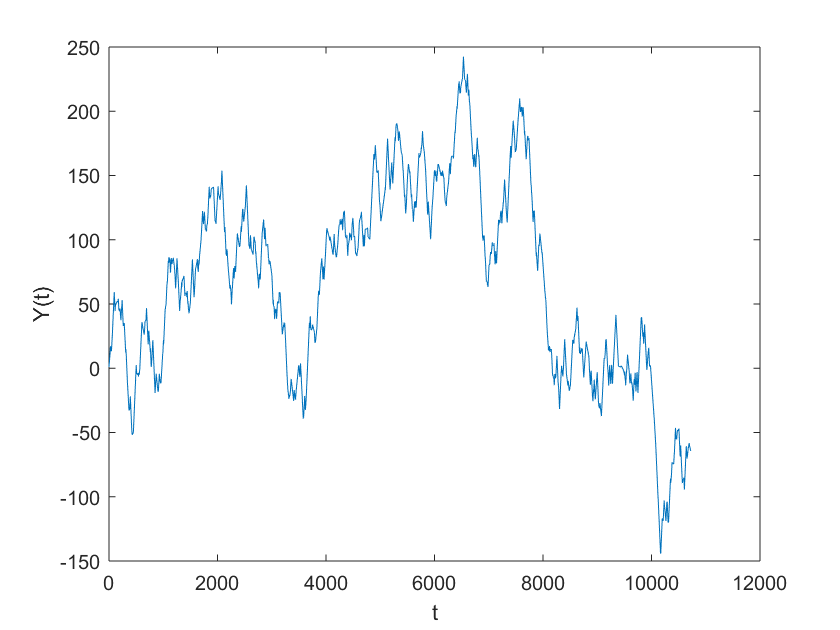
\includegraphics[scale=0.4]{images/N1000T1n10.png}
     \caption{Figure 1}\label{fig:figA}
   \end{subfigure}
   \begin{subfigure}{0.6\linewidth} \centering
     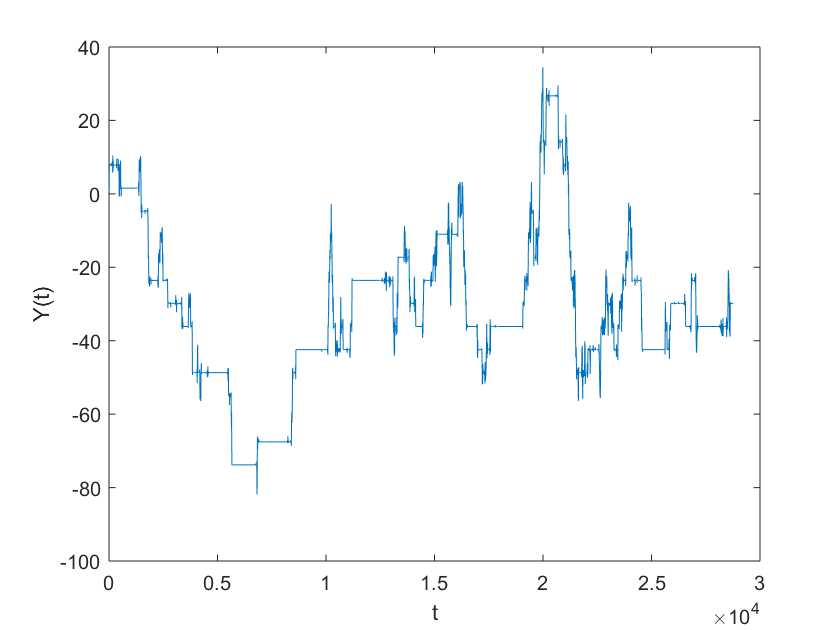
\includegraphics[scale=0.4]{images/N10000T70n20.png}
     \caption{Figure 2}\label{fig:figB}
   \end{subfigure}
\caption{Trajectories of the numerical solution obtained by the Euler-Poisson Scheme} \label{fig:twofigs}
\end{figure}

%We simulated the Euler-Poisson scheme \eqref{eq5} 1000 times sampling from the distribution of $\Delta X_{\xi_{i}(n/T)}$ and chose $a(x)= \sin{(x)}$ arbitrarily with $T=1$, $n=10$.

% \noindent
% Some cross-references: First, we refer to Figure~\ref{fig:twofigs}. 
% Second, we can also refer to the component figures individually, 
% viz., to Figures~\ref{fig:figA} and \ref{fig:figB}.
% \begin{figure}[h]
% \caption{Trajectories of the Euler-Poisson Scheme}
% \centering
% 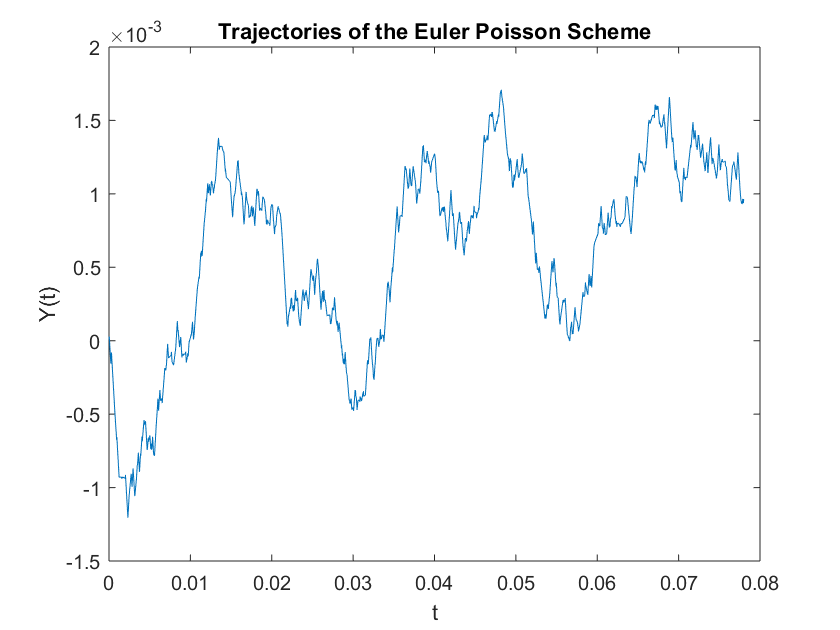
\includegraphics[width=1\textwidth]{images/1000.png}
% \end{figure}

% \begin{figure}[h]
% \caption{Trajectories of the Euler-Poisson Scheme}
% \centering
% 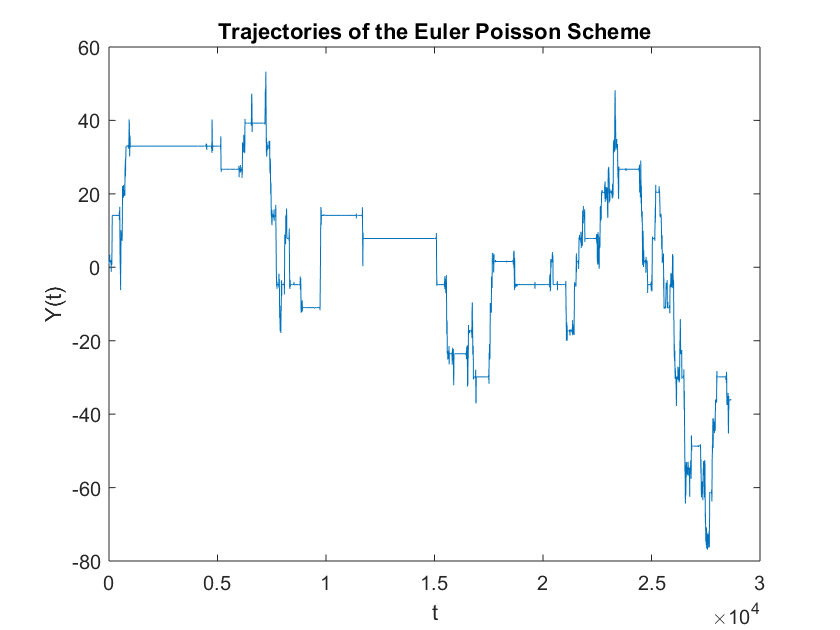
\includegraphics[width=1\textwidth]{images/unscaledN10000T70n20.png}
% \end{figure}